\section{CONTRACTS}

\subsection{Standard 108\th Contracts}

Contracts are established in order to reduce briefing times, increase radio
brevity, remove ambiguity, and increase speed and efficiency. Use them as best
as you can. Contracts can be overridden in briefings and should be done so
\textbf{sparingly} and with good reason.

\textbf{The standard contract in decisions of side, position, azimuth, range
that is used in 108\th will be}

{
    \begin{subsectionenumerate}
    \setlength{\topsep}{0em}

    \item \textbf{Azimuth, Range, Altitude} are taken in order depending on how
      relevant the item is

    \item Leader takes/positions/targets/scans Leftmost first, then nearest if
      not presented in Azimuth, then Highest if no Azimuth or Range makes
      sense, in that order.

    \item \#2 takes "Rightmost first, then Trail, then Low" in order.

    \item \#3, \#4 contracts will need to be defined and prebriefed.

    \item "Left, Lead, High" "Right, Trail, low"\\[1em]

    \end{subsectionenumerate}

    \vspace{-2em}
    This mechanic can be used for
    \setlength{\parskip}{0em}

    \begin{subsectionenumerate}
      \setcounter{enumi}{5}
      \item Standard positioning and formation

      \item Deconfliction direction

      \item Sorting of targets (air and ground)

      \item Firing order
    \end{subsectionenumerate}
}

\subsubsection{Bullseye Contract}
\label{subsubsec:contract-bullseye}

All crews shall set their \textbf{DEF PT} (defended point) to BULLSEYE.
This will allow pilots to quickly select the \textbf{MAN} destination steering
point and read their precise bullseye position when flying with Jester. Please
note, you need to read the reciprocal of the heading needle.

For a named bullseye MARY; If the steer point destination needle points to the
NORTH with 50 nm to go, you will read your position as \textbf{"MARY, one eight
zero (degrees), five zero (miles)"}.

The NAVGRID \textbf{YY} will also be set to Bullseye for easy reference,
however the above will assist with giving your precise position when asked,
especially when flying with Jester.

\textbf{FIX PT} can be used for INS alignment during mission or added
flexibility as an additional waypoint.

\subsection{Pilot RIO contracts}

All contracts can be changed by the Mission Commander in briefing. The
following contracts will remain a default and require to be specifically
overridden.

\newpage

\subsubsection{Comms Contract}

Radios shall be set to Forward - Flight, Rear - Tactical and ATC. RIO should
anticipate agency changes

\begin{itemize}

  \item RIO will control ATC requests and clearances including Carrier Marshall
    and LSO although this duty can be delegated or shared. Pilots must be
    capable of doing this, in the case of single crewed training.

  \item RIO has control of Tactical radio during the Radar Intercept phase
    (Strike, AWACS, AIC)

  \item Pilot has control during the visual arena (Flight control, ACM)

    \begin{itemize}

      \item \textbf{Possible Exception}, the Mission Commander has control of
        flight coordination from a tactical point of view but he can normally
        relay flight controls to the pilot (if he is the RIO) to keep the voice
        consistent on the voice comms

      \item \textbf{Pilot retains flight coordination inside of ACM}

      \item \textbf{RIO moves to "SA informative calls" of working during ACM
        and uses ICS to aid his Pilot}

    \end{itemize}

  \item RIO has control over CAS and FAC(A) transmissions

  \item Pilot will respond to movement directives in the flight

  \item Pilot will handle his flight radio as the voice of the aircraft

  \item RIO will respond to engagement and tactical directives in flight

\end{itemize}

\subsubsection{Firing/Stores Jettison contract}

Pilot has control over weapons with the following exceptions

\begin{itemize}

  \item AIM-54 firing is Primarily RIO. 'Delegation' is discouraged as it leads
    to confusion

  \item The words, "Steady Up!" on ICS should be used to confirm preparation
    for firing (wings level, 1G)

  \item AIM-7 firing is primarily RIO unless the Pilot is using PLM and ACM
    modes visually.

  \item Pilot will direct Fuel and stores jettison

  \item Stores and fuel jettisons are emergency procedures only

  \item Fuel Tanks will always be taken and kept

\end{itemize}

\subsubsection{Radar and combat contract}
\label{sec:radar-and-combat-contract}

The Mission Commander will have control of

\begin{itemize}
  \item Tactical decisions affecting the outcome of the mission
  \item Committal/engagement
  \item Mission 'go, no-go'
\end{itemize}

The RIO will have control of

\begin{itemize}

  \item The Radar, unless it has been transferred to the Pilot over ICS: "Your
  radar" / "My Radar"

  \item The intercept parameters

\end{itemize}

The Pilot will take control of

\begin{itemize}

  \item The Radar when the RIO calls "Your Radar"

  \item The Radar when tally

  \item The Radar in any exceptional visual based requirement, by calling
  \textbf{ICS:} "My Radar" and selecting the relevant PLM mode

  \item Relinquishing the radar with "Your Radar" as soon as practical by
  resetting his scan twice.

\end{itemize}

\subsubsection{Ejection contract}

The RIO shall always set the ejection command selector \textbf{EJECT CMD} to
\textbf{MCO} by drawing it \textbf{aft} during startup to ensure that both crew
members are ejected regardless of who initiated the ejection. This shall be
verbally verify with RIO during cross-checks as the Pilot's EJECT
CMD indicator on the left vertical console is currently inoperable.

\subsubsection{Start up (silent, basic contract)}

To ease excessive verbosity on ICS, the exceptions to silence will be as
follows:

\begin{itemize}
  \item ICS comms check (both)

  \item Ejection safety pin arming (RIO) manual report and readback

  \item Loadout confirmation (Pilot)

  \item Notify RIO when left Engine started and Ground Power off, as signal to
    start the Alignment (Pilot)

  \item Alignment complete (RIO)

  \item RIO ready to taxi (RIO)

  \item Pilot ready to taxi \& all checks complete (Pilot)

\end{itemize}

\subsubsection{Callouts}

RIO shall actively assist with

\begin{itemize}

  \item Landing callouts

  \item Takeoff final checks and speed checks

  \item FENCE cross checks

  \item Ops checks

  \item SA calls

  \item ACM callouts on speed, bandit sightings

  \item Any relevant tactical considerations

  \item Any useful items

  \item ICS is to be considered as a radio in terms of brevity to avoid over
    talking important messages

\end{itemize}

\subsection{FLIGHT CONTRACTS}

\subsubsection{Formation and movement Contract}

The formation and positional contracts are:

\begin{itemize}
  \item Lineup (airfield) Lead takes the downwind (Leeward) side in any
    crosswind, otherwise the far side from the taxiway

  \item Climb: for rejoin 300 KIAS at <95\% RPM. The reduced RPM provides the
    wingman with the excess energy required to intercept the lead aircraft.

  \item Rejoin is Finger four left.

  \item Cruise: AoE Cruise indicator

  \item Air combat readiness: M0.9, combat spread, 1000' vertical
    separation, energy sustaining turns

  \item Tactical Turns of 90 degrees or more should use MIL power

  \item Small check and in place turns should require no change in throttle
    setting

  \item A Fuel Flow of 3000pph is a good cruise setting, or use 8.5 units AoA

  \item When in formation, lead MUST restrict MIL power to <100\% RPM, even in
    climbs. This is to ensure that the wingman has enough excess power
    available to maintain proper formation positioning. During descent, or when
    speedbreaks ("boards") are called to be deployed, lead should avoid
    using idle thrust or risk the wingman overshooting.

\end{itemize}

\subsubsection{Sort \& Scan Contracts}
\label{sec:contracts-sort-scan}

\textbf{"Left, Lead, High - Right, Trail, Low"}

Visual scanning is conducted by both mutually supporting fighters in all
directions with emphasis on looking "through" the other fighter and their blind
spots. This is part of the scan contracts.

Radar scanning should be achieved by mating radars at 20nm at the current
altitude and for the Lead to scan far and high and Wing to scan near and low.

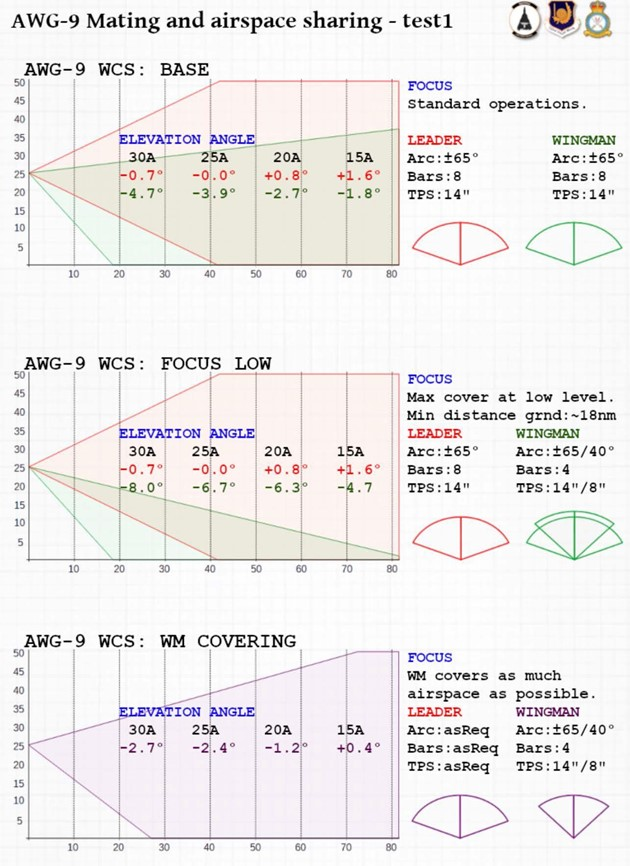
\includegraphics[width=\textwidth]{bvr/radar-mating}

The Tomcat also offers a 360-degree view of the aerial situation around the
aircraft by displaying data-link contacts. If datalink feed is available, this
should be used by both crew members to build and maintain SA, e.g. by selecting
GND STAB or by setting an HCU Offset when turning away from own radar contacts,
to see what's going on outside own radar coverage.

\newpage

\subsubsection{Lost Wingman Procedures}

Holding formation is the WM's responsibility. When visual contact is lost, the
WM must call 'blind'. If FL is visual, he shall assist by stating their
position relative to lost WM: "\textit{1 is visual, your 3 o'clock high}". If
both are blind, the FL shall assist with re-stating heading, altitude and speed.

The A-A TACAN (Yardstick) should be up and running in all phases of the flight
unless required for navigation. If the flight is not separated by more than few
miles, and the tactical situation allows it, WM can ask FL for a flare, or
contrails could be used for assisted visual re-join.

If the flight is separated beyond visual range, the easiest way is to ask
AWACs (if available) for SNAP to the other flight member. Ideally, it should be
the lost WM who is requesting a snap to their FL. The information provided by
AWACS should allow the lost WM to identify their FL with their own radar or
datalink feed to enable a rejoin procedure. It is mandatory that all pilots
(regardless of Jester or RIO) know how to interpret and use the datalink and
work out how to adjust radar range. At minimum radar range, the datalink is a
powerful tool to work out the final intercept geometry for a good rejoin.

If AWACS is not available to provide snap to the other flight member, lead can
immediately relay their position by either using a BULLSEYE reference or an
offset to any TACAN station.

Important, a fix point from Bulls or TACAN is given as your position FROM the
station. As an example, if you are 50 nautical miles NORTH of the Carrier
TACAN, you would give your position as '180 for 50 from mother', so you read
the reciprocal of your Tacan needle.

Using this method, FL can at any time and with an instant read and convey their
current position from Bullseye (see \fullref{subsubsec:contract-bullseye}) or
from any TACAN station (simply rotate the course nob until your radial is
displayed and read the reciprocal of the needle), and this can be used as
reference for rejoining. It is mandatory that all crews practice reading their
Bullseye or Tacan positions, as well as navigating to such a given position for
fast and reliable rejoins.

In order to work out an efficient and expeditious rejoin, it is advisable to
ensure weapons safe and lock up the joined flight member in STT to get precise
distance, closure and drift directly interpretable by the own ship pilot.

Upon penetration of clouds (in situations where a tight fingertip formation is
not feasible), it is equally advisable to use STT locks on the respective
preceding flight member to establish a "Radar-Trail Formation" in order to
proactively prevent a lost-wingman situation.

Navigational (not tactical) radar-trail spacing between aircraft should be kept
between min. 0,5 NM (safety, reaction time) and max. 3 NM (airspace used, ATC
problem avoidance; based on a 30-sec. brake release interval for a departure in
IMC).

In case a joined/trailed flight member complains about the RWR warning tone
caused by his Buddy's Lock, that's what the ALR-67 audio volume knob is for.